\documentclass[10pt]{article}
% Shared preamble of the problems/MHD/setup_notes documents.
% Each case document does % Shared preamble of the problems/MHD/setup_notes documents.
% Each case document does % Shared preamble of the problems/MHD/setup_notes documents.
% Each case document does \input{preamble} right after \documentclass.
\usepackage[margin=0.85in]{geometry}
\usepackage[T1]{fontenc}
\usepackage{lmodern}
\usepackage{amsmath,amssymb,bm}
\usepackage{array,booktabs,tabularx,longtable,multirow}
\usepackage{xcolor}
\usepackage{enumitem}
\usepackage[normalem]{ulem}
\usepackage[hyphens]{url}
\usepackage[colorlinks=true,linkcolor=blue!50!black,urlcolor=blue!50!black]{hyperref}
\usepackage{caption}
\usepackage{graphicx}
\setlist{itemsep=1pt,topsep=3pt}
\sloppy
\emergencystretch=3em
\newcolumntype{Y}{>{\raggedright\arraybackslash}X}
\newcolumntype{L}[1]{>{\raggedright\arraybackslash}p{#1}}

% \code{...}: typewriter with breakable underscores (write \_ in the argument).
\makeatletter
\newcommand{\code}[1]{{\def\_{\char`\_\discretionary{}{}{}}\texttt{#1}}}
\makeatother

% --- Common-item marks -------------------------------------------------------
% \cm{x}  solid underline : identical in EVERY case to which the item applies
% \mj{x}  dashed underline: shared by a MAJORITY of those cases, but not all
\newcommand{\cm}[1]{\uline{#1}}
\newcommand{\mj}[1]{\dashuline{#1}}

\newcommand{\commonlegend}{%
\begin{center}
\fcolorbox{black!40}{black!3}{\parbox{0.92\textwidth}{\small
\textbf{How to read the underlines.}
\cm{Solid underline}: the setting (or the code path) is \emph{identical in every case
of \code{problems/MHD} to which it applies} --- all nine cases for general settings, the eight
\code{DSGS\_MHD} cases for DynSGS settings, the three \code{:positivity\_method => "conservative"}
cases for the element limiter.
\mj{Dashed underline}: shared by a \emph{majority} of those cases but not all of them.
No underline: specific to this case or to a minority.
The cross-case comparison is in \code{summary.pdf} of this directory.}}
\end{center}}

% --- Notation ----------------------------------------------------------------
\newcommand{\bq}{\mathbf{q}}
\newcommand{\bv}{\mathbf{v}}
\newcommand{\bmom}{\mathbf{m}}
\newcommand{\bB}{\mathbf{B}}
\newcommand{\bF}{\mathbf{F}}
\newcommand{\Et}{\tilde E}
\newcommand{\eps}{\varepsilon}
\newcommand{\dsgs}{DynSGS}
\newcommand{\CR}{C_R}
\newcommand{\Cmax}{C_{\max}}
\newcommand{\Cmin}{C_{\min}}
\newcommand{\nuc}{\nu_{c}}
\newcommand{\nufl}{\nu_{\mathrm{fl}}}
\newcommand{\commit}{\code{dcc3653}}
\newcommand{\branch}{\code{sm/MHD}}

% Two-column "setting" table: key | value as used | where / remark
\newenvironment{keytable}{%
\par\smallskip\noindent\small
\begin{longtable}{@{}L{0.24\textwidth}L{0.38\textwidth}L{0.32\textwidth}@{}}
\toprule
\textbf{Deck key / item} & \textbf{Value as run} & \textbf{Source / remark}\\
\midrule\endhead
\bottomrule\endfoot}{%
\end{longtable}\par}
 right after \documentclass.
\usepackage[margin=0.85in]{geometry}
\usepackage[T1]{fontenc}
\usepackage{lmodern}
\usepackage{amsmath,amssymb,bm}
\usepackage{array,booktabs,tabularx,longtable,multirow}
\usepackage{xcolor}
\usepackage{enumitem}
\usepackage[normalem]{ulem}
\usepackage[hyphens]{url}
\usepackage[colorlinks=true,linkcolor=blue!50!black,urlcolor=blue!50!black]{hyperref}
\usepackage{caption}
\usepackage{graphicx}
\setlist{itemsep=1pt,topsep=3pt}
\sloppy
\emergencystretch=3em
\newcolumntype{Y}{>{\raggedright\arraybackslash}X}
\newcolumntype{L}[1]{>{\raggedright\arraybackslash}p{#1}}

% \code{...}: typewriter with breakable underscores (write \_ in the argument).
\makeatletter
\newcommand{\code}[1]{{\def\_{\char`\_\discretionary{}{}{}}\texttt{#1}}}
\makeatother

% --- Common-item marks -------------------------------------------------------
% \cm{x}  solid underline : identical in EVERY case to which the item applies
% \mj{x}  dashed underline: shared by a MAJORITY of those cases, but not all
\newcommand{\cm}[1]{\uline{#1}}
\newcommand{\mj}[1]{\dashuline{#1}}

\newcommand{\commonlegend}{%
\begin{center}
\fcolorbox{black!40}{black!3}{\parbox{0.92\textwidth}{\small
\textbf{How to read the underlines.}
\cm{Solid underline}: the setting (or the code path) is \emph{identical in every case
of \code{problems/MHD} to which it applies} --- all nine cases for general settings, the eight
\code{DSGS\_MHD} cases for DynSGS settings, the three \code{:positivity\_method => "conservative"}
cases for the element limiter.
\mj{Dashed underline}: shared by a \emph{majority} of those cases but not all of them.
No underline: specific to this case or to a minority.
The cross-case comparison is in \code{summary.pdf} of this directory.}}
\end{center}}

% --- Notation ----------------------------------------------------------------
\newcommand{\bq}{\mathbf{q}}
\newcommand{\bv}{\mathbf{v}}
\newcommand{\bmom}{\mathbf{m}}
\newcommand{\bB}{\mathbf{B}}
\newcommand{\bF}{\mathbf{F}}
\newcommand{\Et}{\tilde E}
\newcommand{\eps}{\varepsilon}
\newcommand{\dsgs}{DynSGS}
\newcommand{\CR}{C_R}
\newcommand{\Cmax}{C_{\max}}
\newcommand{\Cmin}{C_{\min}}
\newcommand{\nuc}{\nu_{c}}
\newcommand{\nufl}{\nu_{\mathrm{fl}}}
\newcommand{\commit}{\code{dcc3653}}
\newcommand{\branch}{\code{sm/MHD}}

% Two-column "setting" table: key | value as used | where / remark
\newenvironment{keytable}{%
\par\smallskip\noindent\small
\begin{longtable}{@{}L{0.24\textwidth}L{0.38\textwidth}L{0.32\textwidth}@{}}
\toprule
\textbf{Deck key / item} & \textbf{Value as run} & \textbf{Source / remark}\\
\midrule\endhead
\bottomrule\endfoot}{%
\end{longtable}\par}
 right after \documentclass.
\usepackage[margin=0.85in]{geometry}
\usepackage[T1]{fontenc}
\usepackage{lmodern}
\usepackage{amsmath,amssymb,bm}
\usepackage{array,booktabs,tabularx,longtable,multirow}
\usepackage{xcolor}
\usepackage{enumitem}
\usepackage[normalem]{ulem}
\usepackage[hyphens]{url}
\usepackage[colorlinks=true,linkcolor=blue!50!black,urlcolor=blue!50!black]{hyperref}
\usepackage{caption}
\usepackage{graphicx}
\setlist{itemsep=1pt,topsep=3pt}
\sloppy
\emergencystretch=3em
\newcolumntype{Y}{>{\raggedright\arraybackslash}X}
\newcolumntype{L}[1]{>{\raggedright\arraybackslash}p{#1}}

% \code{...}: typewriter with breakable underscores (write \_ in the argument).
\makeatletter
\newcommand{\code}[1]{{\def\_{\char`\_\discretionary{}{}{}}\texttt{#1}}}
\makeatother

% --- Common-item marks -------------------------------------------------------
% \cm{x}  solid underline : identical in EVERY case to which the item applies
% \mj{x}  dashed underline: shared by a MAJORITY of those cases, but not all
\newcommand{\cm}[1]{\uline{#1}}
\newcommand{\mj}[1]{\dashuline{#1}}

\newcommand{\commonlegend}{%
\begin{center}
\fcolorbox{black!40}{black!3}{\parbox{0.92\textwidth}{\small
\textbf{How to read the underlines.}
\cm{Solid underline}: the setting (or the code path) is \emph{identical in every case
of \code{problems/MHD} to which it applies} --- all nine cases for general settings, the eight
\code{DSGS\_MHD} cases for DynSGS settings, the three \code{:positivity\_method => "conservative"}
cases for the element limiter.
\mj{Dashed underline}: shared by a \emph{majority} of those cases but not all of them.
No underline: specific to this case or to a minority.
The cross-case comparison is in \code{summary.pdf} of this directory.}}
\end{center}}

% --- Notation ----------------------------------------------------------------
\newcommand{\bq}{\mathbf{q}}
\newcommand{\bv}{\mathbf{v}}
\newcommand{\bmom}{\mathbf{m}}
\newcommand{\bB}{\mathbf{B}}
\newcommand{\bF}{\mathbf{F}}
\newcommand{\Et}{\tilde E}
\newcommand{\eps}{\varepsilon}
\newcommand{\dsgs}{DynSGS}
\newcommand{\CR}{C_R}
\newcommand{\Cmax}{C_{\max}}
\newcommand{\Cmin}{C_{\min}}
\newcommand{\nuc}{\nu_{c}}
\newcommand{\nufl}{\nu_{\mathrm{fl}}}
\newcommand{\commit}{\code{dcc3653}}
\newcommand{\branch}{\code{sm/MHD}}

% Two-column "setting" table: key | value as used | where / remark
\newenvironment{keytable}{%
\par\smallskip\noindent\small
\begin{longtable}{@{}L{0.24\textwidth}L{0.38\textwidth}L{0.32\textwidth}@{}}
\toprule
\textbf{Deck key / item} & \textbf{Value as run} & \textbf{Source / remark}\\
\midrule\endhead
\bottomrule\endfoot}{%
\end{longtable}\par}

\newgeometry{margin=0.62in,top=0.5in,bottom=0.55in}
\captionsetup{font=small,labelfont=bf,skip=3pt}
\setlength{\parskip}{3pt}
\setlength{\parindent}{0pt}
\pagestyle{empty}
\begin{document}

{\Large\bfseries DynSGS without and with the smoothness cutoff $c=10^{-3}$}\\[2pt]
{\small Measured on the smooth Alfv\'en wave (\code{problems/MHD/alfvenWaveBabbarRanocha2026}, Babbar \& Ranocha 2026,
\S5.5.1), branch \branch{}, commit \code{e40bc3e}. The cutoff is the deck entry \code{AW\_CUTOFF} (\code{:dsgs\_cutoff}),
$10^{-3}$ by default.}

\vspace{-2pt}\noindent\rule{\textwidth}{0.4pt}

\textbf{The coefficient.} On element $K$, with $\Delta_K=\Delta^{elem}_K/(N+1)$ and $w_K=\max(|\bv|+c_f)$,
\[
\nu_K=\min\!\big(\Cmax\,\Delta_K\,w_K,\ \ \CR\,\Delta_K^2\,\max(0,\ r_K-c)\big),\qquad
r_K=\max_i\frac{\|R_i\|_{\infty,K}}{n_i},\qquad R=\partial_t\bq+\nabla\!\cdot\bF(\bq),
\]
$R$ being the element's own strong residual and $n_i$ the domain-wide scale of variable $i$ (its spread, floored at the
physical scale; here $\bar\rho\bar c=0.42$ for the momentum and $\bB$). $\CR=1$, $\Cmax=0.5$, $\Cmin=0$.
\textbf{Without the cutoff} is $c=0$: $\nu_K=\CR\Delta_K^2 r_K$, whatever $r_K$ is. \textbf{With it}, $c=10^{-3}$ is
subtracted from the normalized residual first, so $\nu_K=0$ wherever $r_K\le10^{-3}$, and $\nu_K$ stays continuous across
the threshold (it is not an on/off switch).

\begin{minipage}[t]{0.52\textwidth}
\textbf{Without the cutoff: a floor that converges at order 4.} The coefficient is computed once per step, and the
$\partial_t\bq$ in $R$ is the BDF2 of three step-level states, whose truncation error is $\tfrac{\Delta t^2}{3}\partial_t^3\bq$.
On a resolved smooth solution the spatial part of $R$ is $O(h^N)$, but a travelling wave has
$\partial_t^3\bq=\omega^3A\neq0$ however well it is resolved ($\omega=2\pi$, $A=0.1$). So $r_K$ never falls below
\[
r_{\rm floor}=\frac{\Delta t^2}{3}\,\frac{\omega^3A}{\bar\rho\bar c}\quad(4\cdot10^{-6}\ \text{to}\ 7\cdot10^{-4}\ \text{over the sweep}),
\]
and $\nu\approx\CR\Delta^2 r_{\rm floor}\propto\Delta^2\Delta t^2\propto h^4$ at a fixed Courant number,
\emph{whatever $N$}. That $\nu$ damps the wave by $\nu k^2t$ ($k=2\pi$), a state error of $0.14\,\nu k^2 t$:
\begin{itemize}[leftmargin=12pt]
\item it predicts the measured error with no fitted constant ($N=6$ on $16^2$: $5.4\cdot10^{-8}$ predicted and
measured; $N=5,6,7$ within $0.95$--$1.4\times$ from $8^2$ on);
\item DynSGS converges at $\approx4$ for $N=5,6,7$, and at equal \#DOFs the three curves coincide, since $\Delta$ and
$\Delta t$ are both set by the node spacing;
\item halving $\Delta t$ alone divides the error by $3.9$--$4.0$, and the Galerkin error does not move;
\item at $N=3$ the floor is ${\sim}1/100$ of Galerkin's own error, and does not show.
\end{itemize}
\textbf{With the cutoff $c=10^{-3}$.} $r_{\rm floor}<10^{-3}$ on every mesh of the sweep, so $\nu\equiv0$ and DynSGS
\emph{is} the Galerkin scheme: bit for bit, all nine variables, $L^2$ and $L^\infty$, for $N=5,6,7$ on every mesh but
the coarsest of $N=5$. The orders are Galerkin's (6.5, 6.0, 8.6 on the finest pair). Where the residual is real
the cutoff barely matters: at a discontinuity $r_K=O(10^2)$, which $c$ changes by $10^{-5}$ relative.
\end{minipage}\hfill
\begin{minipage}[t]{0.455\textwidth}
\vspace{2pt}
\centering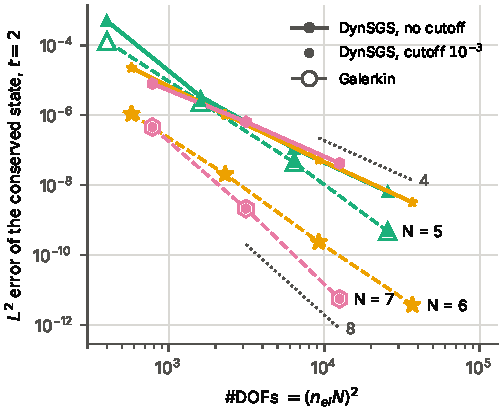
\includegraphics[width=\linewidth]{dsgsCutoff_fig.pdf}
\captionof{figure}{State error at $t=2$, $N=5,6,7$. Solid: DynSGS without the cutoff (slope 4). Small filled
markers inside the hollow Galerkin ones: DynSGS with $c=10^{-3}$, identical to Galerkin.}
\vspace{4pt}
{\footnotesize\setlength{\tabcolsep}{3.2pt}
\begin{tabular}{@{}cc|cc|cc|cc@{}}
\toprule
$N$ & mesh & \multicolumn{2}{c|}{no cutoff} & \multicolumn{2}{c|}{$c=10^{-3}$} & \multicolumn{2}{c}{Galerkin}\\
\midrule
5 & $8^2$  & 3.4e-6 & & 2.4e-6 & & 2.4e-6 & \\
5 & $16^2$ & 1.1e-7 & 5.0 & 4.4e-8 & 5.8 & 4.4e-8 & 5.8\\
5 & $32^2$ & 6.4e-9 & 4.1 & 4.8e-10 & 6.5 & 4.8e-10 & 6.5\\
6 & $8^2$  & 1.0e-6 & & 2.0e-8 & & 2.0e-8 & \\
6 & $16^2$ & 5.4e-8 & 4.3 & 2.4e-10 & 6.4 & 2.4e-10 & 6.4\\
6 & $32^2$ & 3.2e-9 & 4.1 & 3.7e-12 & 6.0 & 3.7e-12 & 6.0\\
7 & $8^2$  & 6.5e-7 & & 2.1e-9 & & 2.1e-9 & \\
7 & $16^2$ & 4.2e-8 & 3.9 & 5.5e-12 & 8.6 & 5.5e-12 & 8.6\\
\bottomrule
\end{tabular}}
\captionof{table}{State $L^2$ error and order.}
\end{minipage}

\vspace{4pt}
\textbf{What the cutoff does \emph{not} settle.}
\begin{itemize}[leftmargin=12pt]
\item \emph{Under-resolution.} $N=5$ on $4^2$ (20 points per side, the least resolved run): $r_K>10^{-3}$ in places,
$\nu$ up to $9\cdot10^{-5}$, error $3.6\times$ Galerkin's. There the viscosity acts, as it should on a marginal wave.
\item \emph{Shocks.} $c=10^{-3}$ is above this wave's floor on every mesh (at most $7\cdot10^{-4}$) and 5 decades below
a shock's $r_K$, but it has not been run on the shock cases (Brio--Wu, Orszag--Tang, rotor, blast). On the smooth MHD vortex ($N=6$, $32^2$,
$t=0.5$) the cutoff likewise gives Galerkin bit for bit; there the excess without it was only 2\%.
\item \emph{What $10^{-3}$ means.} $c$ is compared with $r_K$, i.e.\ with the residual \emph{divided by} $n_i$: another
normalization (\code{:dsgs\_rel}, element norms) changes the threshold it stands for.
\end{itemize}

\textbf{Reproduce.} \code{tools/alfven\_wave\_scan.sh} runs the deck as committed, $c=10^{-3}$, for $N=3\ldots7$
(\code{AW\_JOBS=5} runs the five orders at once). With \code{AW\_CUTOFF = 0.0} in \code{user\_inputs.jl},
\code{AW\_KEEP=1 AW\_VISC=dsgs tools/alfven\_wave\_scan.sh} adds the curves without the cutoff (records
\code{dsgs\_nocut}). \code{dsgsCutoff\_fig.py} redraws Fig.~1 from the case's error store.

\end{document}
